\documentclass[12pt]{article}
\date{February 23, 2019}
\usepackage{pgf-pie}
\usepackage{pgfplots}
\usepackage{pgfplotstable}
\usetikzlibrary{patterns}
\usepackage[section]{placeins}
\usepackage[utf8]{inputenc}

\begin{document}


\clearpage{}
\section{How old are you?}

\label{sec:1}


\begin{figure}[h!]
    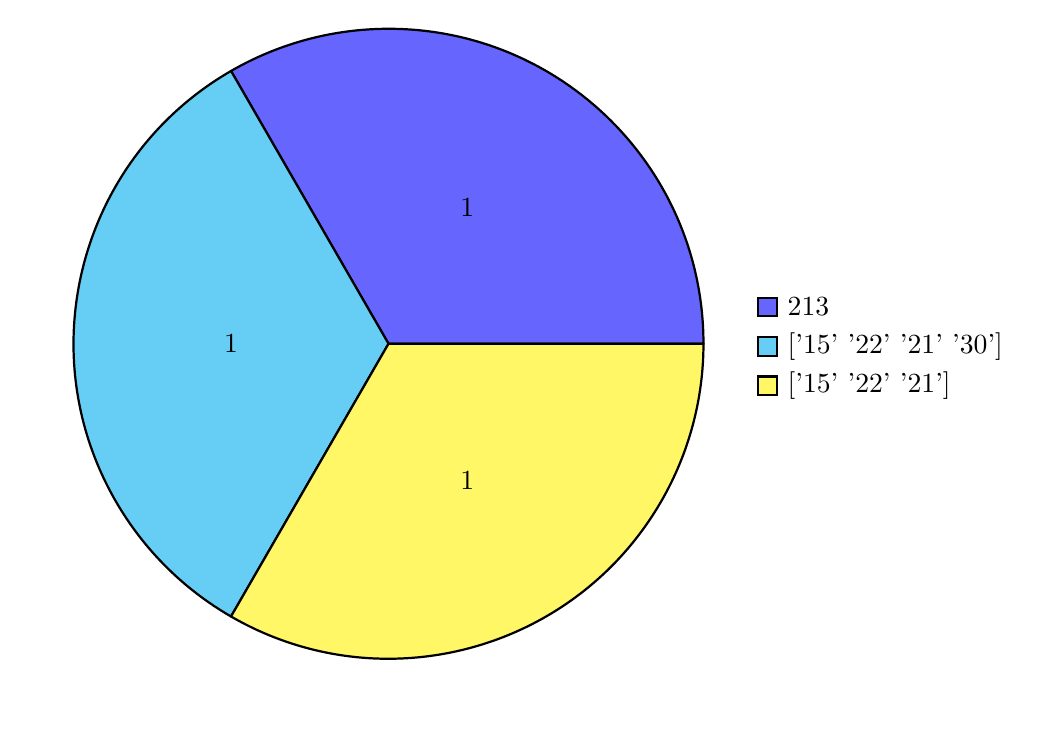
\begin{tikzpicture}
        \pie[radius=4,sum=auto,text=legend]{
            1/213,
            1/['15'  '22'  '21'  '30'],
            1/['15'  '22'  '21']
        }
    \end{tikzpicture}
    \caption{\label{figure:q1-1}Repartition of answers for the question 'How old are you?'.}
\end{figure}



\clearpage{}
\section{What is your name?}

\label{sec:2}


\begin{figure}[h!]
    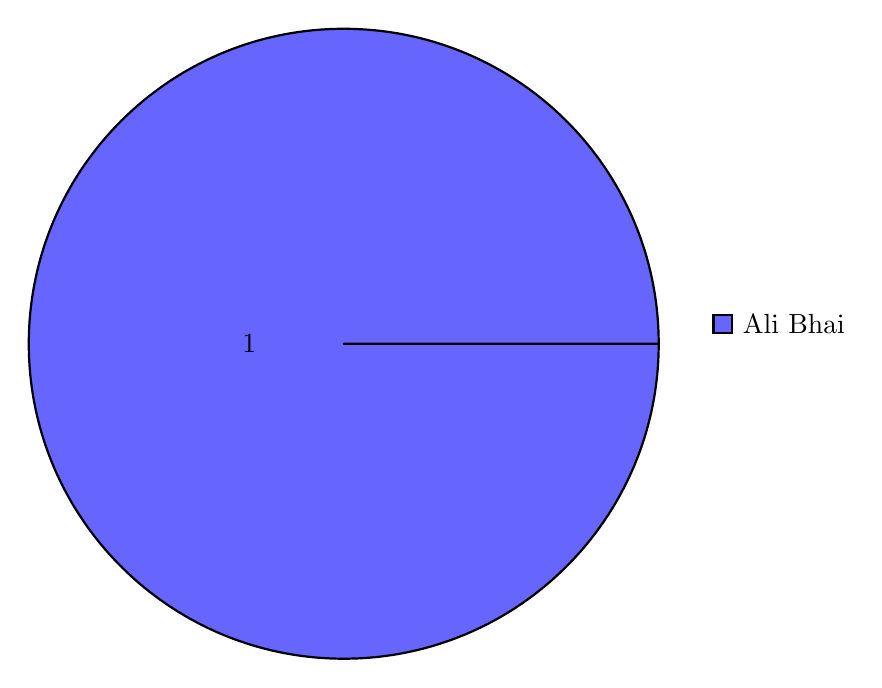
\begin{tikzpicture}
        \pie[radius=4,sum=auto,text=legend]{
            1/Ali Bhai
        }
    \end{tikzpicture}
    \caption{\label{figure:q2-1}Repartition of answers for the question 'What is your name?'.}
\end{figure}



\clearpage{}
\section{Address?}

\label{sec:3}


\begin{figure}[h!]
    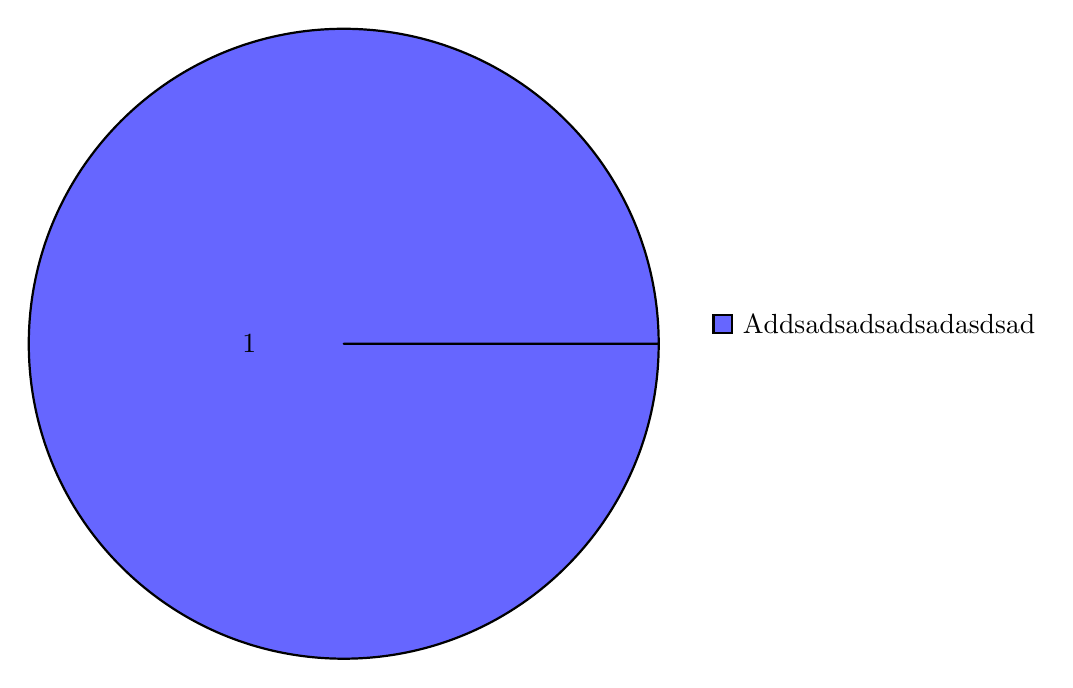
\begin{tikzpicture}
        \pie[radius=4,sum=auto,text=legend]{
            1/Addsadsadsadsadasdsad
        }
    \end{tikzpicture}
    \caption{\label{figure:q3-1}Repartition of answers for the question 'Address?'.}
\end{figure}



\clearpage{}
\section{Somthing}

\label{sec:4}


\begin{figure}[h!]
    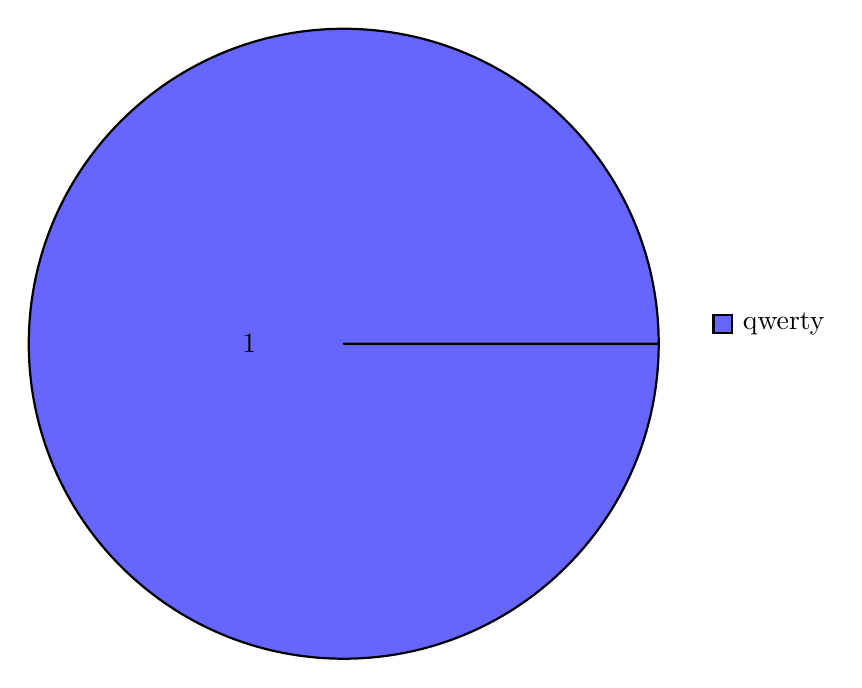
\begin{tikzpicture}
        \pie[radius=4,sum=auto,text=legend]{
            1/qwerty
        }
    \end{tikzpicture}
    \caption{\label{figure:q4-1}Repartition of answers for the question 'Somthing'.}
\end{figure}



\end{document}
